\documentclass[11pt]{article}
% Self-contained (article) so it compiles under MiKTeX without the Springer class.
% At submission (Task 13) port sections into sn-jnl.cls; content is class-agnostic.
\usepackage[utf8]{inputenc}
\usepackage[T1]{fontenc}
\usepackage{lmodern}
\usepackage[margin=1in]{geometry}
\usepackage{booktabs}
\usepackage{graphicx}
\usepackage{amsmath}
\usepackage[table]{xcolor}
\usepackage{tcolorbox}
\definecolor{hlrow}{RGB}{225,238,248}
\usepackage{caption}
\usepackage{algorithm}
\usepackage{algpseudocode}
\usepackage[hidelinks]{hyperref}
\usepackage{natbib}
\bibliographystyle{plainnat}
\graphicspath{{../results/figures/}}

\title{\textbf{TrustShift: Shift Type, Not Shift Magnitude,\\
Determines Machine-Learning Failure Modes}\\
\large A cross-domain audit protocol and a failure taxonomy}
\author{Rajveer Singh Pall}
\date{}

\begin{document}
\maketitle

\begin{abstract}
\noindent Deployment evaluation implicitly assumes that a larger distribution shift means greater
risk. Across four domains, we find this assumption false. We introduce \textbf{TrustShift}, a
single pre-registered protocol measuring discrimination, calibration, and subgroup reliability, and
apply it identically to four real deployment shifts: clinical risk prediction
(NHANES$\rightarrow$BRFSS), mental-health text classification (Kaggle$\rightarrow$Reddit/Twitter),
mortgage-approval prediction (temporal and cross-state shift over 42M U.S.\ loan records), and
network-intrusion detection (CIC-DDoS2019$\rightarrow$CICIDS2017). A lending model under large
measured covariate shift (domain-classifier AUC up to $0.80$) degrades on no axis, while a
mental-health model at comparable magnitudes loses up to $0.39$ AUC: magnitude does not predict
damage. The shift \emph{type} does. Concept shift breaks every axis; novel-label shift blinds a
detector to unseen classes while its in-domain AUC reads a perfect $1.00$; covariate shift alone
breaks nothing; mixed shift breaks calibration silently while discrimination holds. In-domain
metrics anticipated none of this, yet three inexpensive diagnostic probes correctly distinguish the
shift type before deployment. Post-hoc recalibration then cuts calibration error by one to two orders of magnitude in
every domain but never restores lost discrimination or subgroup reliability. We contribute a protocol
and a four-domain benchmark, and distill the result into a failure taxonomy mapping a
pre-deployment diagnosis to the trustworthiness axis at risk.
\end{abstract}

\section{Introduction}\label{sec:intro}

Consider three machine-learning systems at the moment of deployment. A clinical risk model moves
from a survey cohort to a national screening population; its discrimination barely changes, and it
looks fine---yet its probability estimates become substantially miscalibrated, so the risk numbers
it reports are wrong. An intrusion detector moves from one year's attack corpus to the next; its
in-domain AUC is a perfect $1.00$, and it looks flawless---yet it is nearly blind to the attack
families it will actually meet. A mortgage-approval model moves across years and states under a
distribution shift large enough to be detected almost perfectly by a classifier trained to spot
it---and nothing breaks; its accuracy even improves.

Three systems, three intuitions overturned. We argue these are not isolated accidents but three
faces of one deployment phenomenon. The one that looked fine failed; the one that looked perfect
failed; the one that looked most shifted did not. Why? Answering that question is the subject of
this paper, and the answer is not the magnitude of the shift.

Deployment evaluation is dominated by a single in-domain number---accuracy, or AUC---treated as
evidence of readiness. When shift is considered at all, it is treated as a scalar severity: bigger
shift, bigger risk. And it is studied one domain at a time. Clinical prediction has a mature
external-validation literature; fairness-under-shift has been examined in medical
imaging~\citep{schrouff2022diagnosing}; tabular shift has dedicated
benchmarks~\citep{gardner2023tableshift}; general shift benchmarks span vision and
language~\citep{koh2021wilds}. Each answers ``does this model degrade here?'' None answers the
cross-domain question our three vignettes raise: \emph{are deployment failures of trustworthiness
domain-specific accidents, or do they follow rules that hold across domains---and can those rules
be read before deployment?}

We answer it with one protocol applied to four deliberately dissimilar domains (the three above
plus mental-health text classification). The protocol measures three trustworthiness axes
(discrimination, calibration, subgroup reliability), assigns each shift a mechanistic diagnosis
(label, covariate, or concept shift) using cheap and largely label-free probes, and quantifies what
a remediation ladder restores. Holding the protocol fixed across clinical tabular data, social-media
text, mortgage records, and network traffic separates what is general from what is idiosyncratic.
The result is a taxonomy (Figure~\ref{fig:taxonomy}): across these domains the shift type, not its
magnitude, consistently predicts which axis fails, and the shift type is cheap to diagnose in advance.

\paragraph{Contributions.}
\begin{itemize}
  \item \textbf{Shift type, not magnitude, tracks the failure (the discovery).} We show---and expose
  the statistical trap behind---that the \emph{magnitude} of covariate shift does not predict
  deployment damage, while the shift \emph{type} does (Section~\ref{sec:meta}). A lending model at
  large measured shift is robust; a text model at comparable magnitude collapses.
  \item \textbf{A failure taxonomy backed by four domains.} We show that the trustworthiness axis
  that fails is consistently predicted by the shift's mechanistic type across four domains
  (Table~\ref{tab:fingerprint})---turning measurement into classification.
  \item \textbf{A remediation result.} Across all four domains, post-hoc recalibration is the only
  cheap repair and it repairs only calibration; discrimination and subgroup reliability lost to
  shift require target supervision.
  \item \textbf{A protocol, not just a benchmark.} TrustShift is a reusable, pre-registered
  five-quantity audit (discrimination, calibration, subgroup gap, shift diagnosis, remediation)
  that runs identically on any (source, target) prediction pair, generalizing the single-domain
  CPFE protocol~\citep{pall2026cpfe} to a domain-agnostic instrument.
  \item \textbf{A benchmark (available upon publication).} Four harmonized shift-pairs, standardized predictions, and
  the protocol implementation, enabling others to place new domains on the same axes.
\end{itemize}

\begin{figure}[t]
\centering
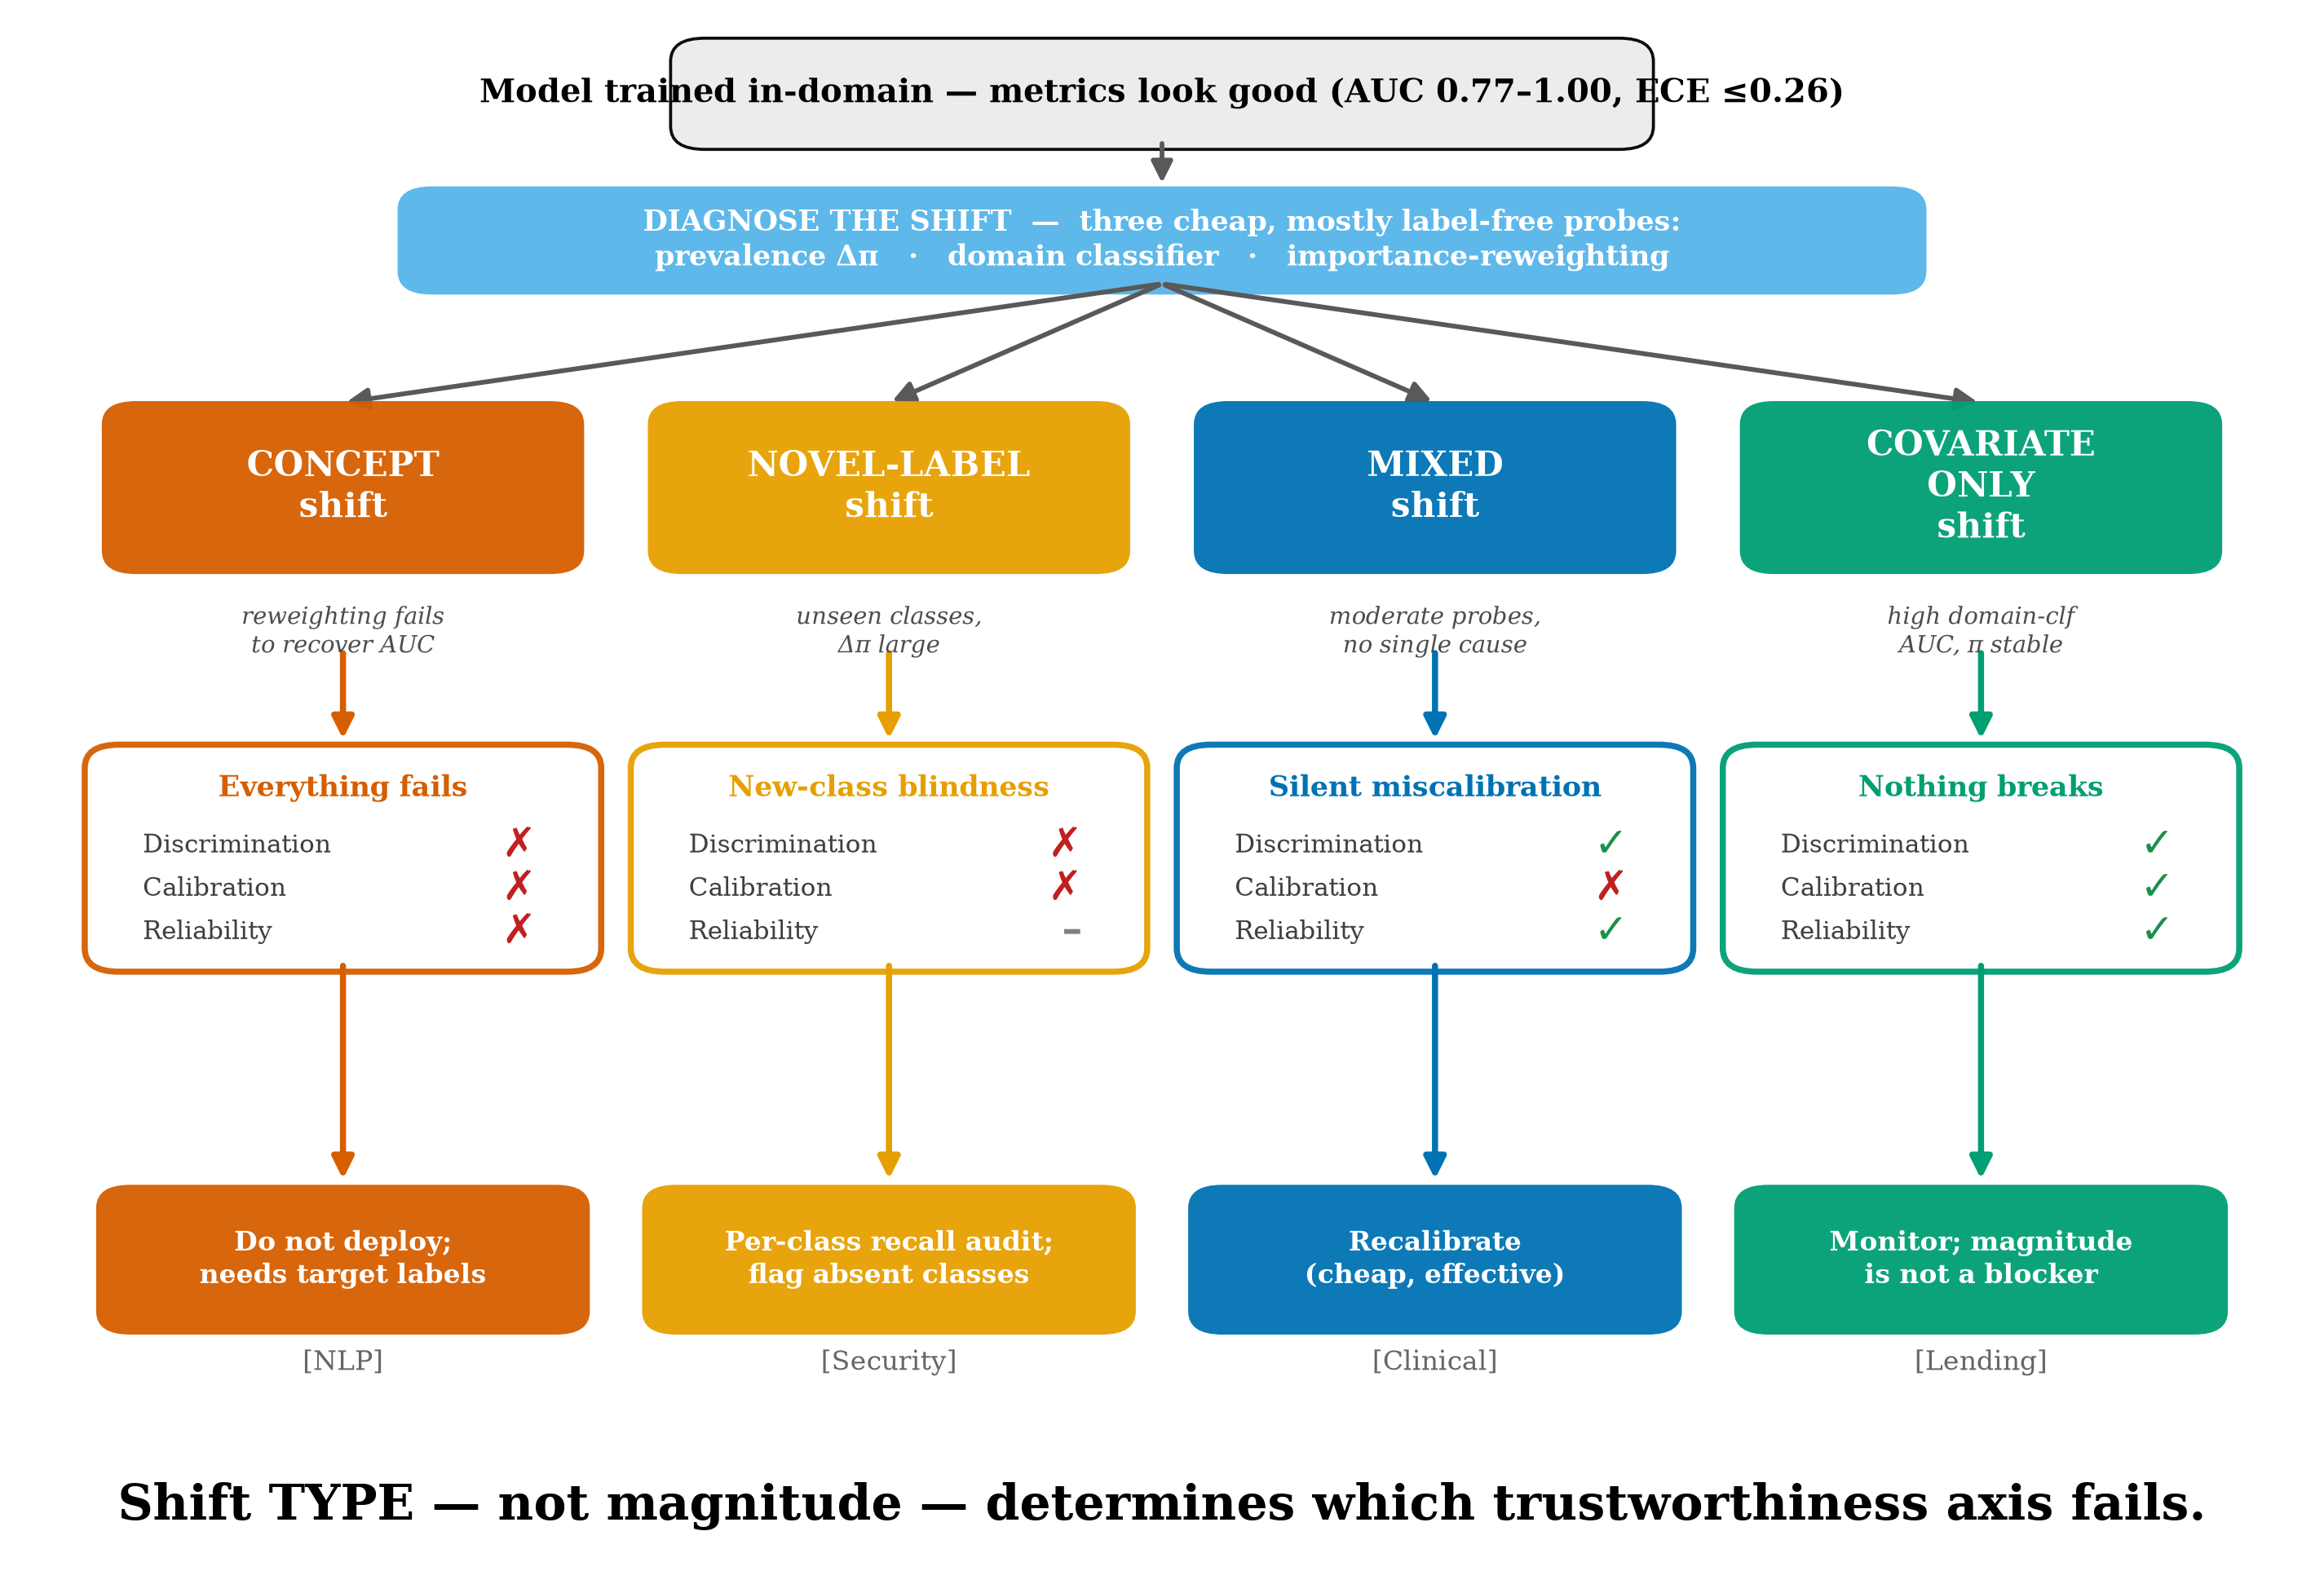
\includegraphics[width=\linewidth]{fig1_taxonomy.png}
\caption{\textbf{The TrustShift failure taxonomy.} A model that looks deployable in-domain (top) is
diagnosed by three cheap, largely label-free probes; the resulting shift type (colored branches)
predicts which trustworthiness axis fails and the audit a practitioner should run. Each branch is
realized by one of our four domains. In-domain metrics predicted none of these outcomes; the shift
type did.}
\label{fig:taxonomy}
\end{figure}

\section{The TrustShift Protocol}\label{sec:protocol}

The protocol consumes, for each domain, a source model's predictions on an in-distribution test
split (\emph{source}) and on one or more deployment splits (\emph{target}), together with a
subgroup label per example. It emits five quantities.

\paragraph{Axis 1: Discrimination.} AUC (macro one-vs-rest for multiclass domains) and macro-F1
per split, with DeLong 95\% confidence intervals~\citep{delong1988comparing}. We report
$\Delta\text{AUC} = \text{AUC}_{\text{source}} - \text{AUC}_{\text{target}}$.

\paragraph{Axis 2: Calibration.} Expected Calibration Error (ECE, 10 equal-width bins) and Brier
score per split. ECE quantifies the gap between predicted confidence and empirical
accuracy~\citep{guo2017calibration}; a model can discriminate perfectly and still be badly
calibrated, and vice versa.

\paragraph{Axis 3: Subgroup reliability.} Per subgroup $g$, AUC$_g$; the subgroup gap
$G(\text{split}) = \max_g \text{AUC}_g - \min_g \text{AUC}_g$; and the \emph{gap change}
$\Delta G = G(\text{target}) - G(\text{source})$---the headline reliability quantity---with a
stratified bootstrap 95\% CI ($N=2000$). Subgroups are demographic where available (clinical:
age, sex, race, BMI; lending: race), platform-derived proxy classes for text, and \emph{operational}
(attack family) for intrusion detection. We call this subgroup-conditional reliability and, for
intrusion detection, never interpret it as demographic fairness (Section~\ref{sec:limitations}).

\paragraph{Axis 4: Shift diagnosis.} Each shift is decomposed with three cheap probes.
\emph{Label shift}: change in class prevalence $\Delta\pi$ (labels only).
\emph{Covariate shift}: a domain classifier trained to separate source from target examples on
shared features, scored by 5-fold cross-validated AUC ($\text{AUC}_{\text{dc}}$; $0.5$ = no shift,
$\rightarrow 1$ = severe)~\citep{rabanser2019failing}.
\emph{Concept shift}: importance-weighting the source examples by the domain-classifier odds and
recomputing source AUC; if the reweighted source AUC stays near the source AUC while the target
AUC is far lower, covariate shift alone cannot explain the drop~\citep{lipton2018label}.

\paragraph{Axis 5: Remediation ladder.} On a 10\% stratified target calibration split we apply
temperature, Platt, and isotonic recalibration~\citep{zadrozny2002isotonic}, then re-measure
Axes 1--3 on the remaining 90\%. This isolates what a cheap post-hoc fix restores from what
requires target supervision.

Full metric definitions, seeds, and estimator choices are fixed in the released configuration;
all reported numbers regenerate from committed prediction files. Algorithm~\ref{alg:trustshift}
states the protocol as executed.

\begin{algorithm}[t]
\caption{The TrustShift audit}
\label{alg:trustshift}
\begin{algorithmic}[1]
\Require source predictions $(\hat p, y, g)_{\text{src}}$; target predictions $(\hat p, y, g)_{\text{tgt}}$; shared features $X_{\text{src}}, X_{\text{tgt}}$
\Statex \textit{\textbf{Stage 1 --- Evaluate the three trustworthiness axes}}
\State $\Delta\text{AUC} \gets \text{AUC}_{\text{src}} - \text{AUC}_{\text{tgt}}$; \; ECE, Brier per split \Comment{DeLong CIs; 10 bins}
\State $\Delta G \gets (\max_g\!-\!\min_g)\text{AUC}_g^{\text{tgt}} - (\max_g\!-\!\min_g)\text{AUC}_g^{\text{src}}$ \Comment{subgroup gap; bootstrap CI}
\Statex \textit{\textbf{Stage 2 --- Diagnose the shift type}}
\State $\Delta\pi \gets$ prevalence change; \; $\text{AUC}_{\text{dc}} \gets$ CV-AUC of a source-vs-target classifier on $X$
\State $w(x) \gets$ domain-classifier odds; \; $\text{AUC}^{\text{rw}}_{\text{src}} \gets$ $w$-weighted source AUC
\If{$\text{AUC}^{\text{rw}}_{\text{src}} \approx \text{AUC}_{\text{src}} \gg \text{AUC}_{\text{tgt}}$} diagnosis $\gets$ \textbf{concept}
\ElsIf{$|\Delta\pi|$ large / unseen classes} diagnosis $\gets$ \textbf{novel-label}
\ElsIf{$\text{AUC}_{\text{dc}} > 0.65$} diagnosis $\gets$ \textbf{covariate} \Else{} diagnosis $\gets$ \textbf{mixed} \EndIf
\Statex \textit{\textbf{Stage 3 --- Remediate and re-measure}}
\State fit recalibration on 10\% target labels; re-measure the three axes on the rest
\Ensure $(\Delta\text{AUC},\, \text{ECE},\, \Delta G,\, \text{diagnosis},\, \text{restored axes})$
\end{algorithmic}
\end{algorithm}

\section{Domains and Data}\label{sec:data}

We chose four domains that differ in modality, subgroup semantics, and shift mechanism, so that
any shared pattern is unlikely to be an artifact of one setting (Table~\ref{tab:data}).

\begin{table}[t]
\centering
\caption{The four deployment shifts. Subgroup semantics deliberately differ; the protocol is
identical.}
\label{tab:data}
\small
\begin{tabular}{lllll}
\toprule
Domain & Source $\rightarrow$ Target & Modality & Subgroup axis & Shift mechanism \\
\midrule
Clinical & NHANES $\rightarrow$ BRFSS & tabular & age/sex/race/BMI & population \\
NLP & Kaggle $\rightarrow$ Reddit, Twitter & text & proxy class & platform/style \\
Lending & HMDA 2020--21 $\rightarrow$ 2022--24; cross-state & tabular & race, income & temporal, geographic \\
Security & CIC-DDoS2019 $\rightarrow$ CICIDS2017 & network flow & attack family & novel attacks \\
\bottomrule
\end{tabular}
\end{table}

The clinical and NLP source models reuse published predictions
(\citealp{pall2026cpfe}, a preprint under review, for NLP, evaluated on GoEmotions~\citep{demszky2020goemotions} and a
Twitter emotion corpus; a diabetes external-validation study on NHANES~\citep{nhanes} and
BRFSS~\citep{brfss} for clinical), so no retraining occurs and the source numbers reproduce prior
work. The lending and security analyses are new: for lending we train gradient-boosted approval
classifiers with no race or geographic feature on HMDA loan records~\citep{hmda} and evaluate
temporal (train 2020--21, test each of 2022/2023/2024) and geographic (train on 60\% of states,
test on held-out states) shift over 42.3M records; for security we train intrusion detectors on
CIC-DDoS2019~\citep{sharafaldin2019ddos2019} and evaluate on
CICIDS2017~\citep{sharafaldin2018ids2017}. Data are public. Clinical target-side subgroup analysis
is limited to age for a reason we state plainly in Section~\ref{sec:limitations}.

\section{Results}\label{sec:results}

We organize results as one argument: in-domain metrics do not predict deployment behaviour
(\ref{sec:res-indomain}); the failure that occurs is consistently predicted by the shift type
across domains (\ref{sec:res-fingerprint}); that regularity is categorical, not a magnitude law
(\ref{sec:meta}); and recalibration repairs only calibration (\ref{sec:res-remediation}).

\subsection{In-domain performance does not transfer, and does not transfer uniformly}
\label{sec:res-indomain}

Every source model looked deployable: source AUC ranged from $0.77$ (clinical) to $1.00$
(security) and source ECE was at most $0.26$. Deployment outcomes did not follow
(Figure~\ref{fig:bars}, Table~\ref{tab:master}). Mental-health classifiers lost $0.28$--$0.39$
AUC on new platforms; the intrusion detector fell from AUC $1.00$ to $0.64$; the clinical model
barely moved in AUC ($0.788\rightarrow 0.757$); and lending models did not degrade at all, in
fact improving slightly on later years. A single in-domain dashboard would have rated all four
identically ``ready.'' None of the deployment outcomes is readable from it.

\begin{figure}[t]
\centering
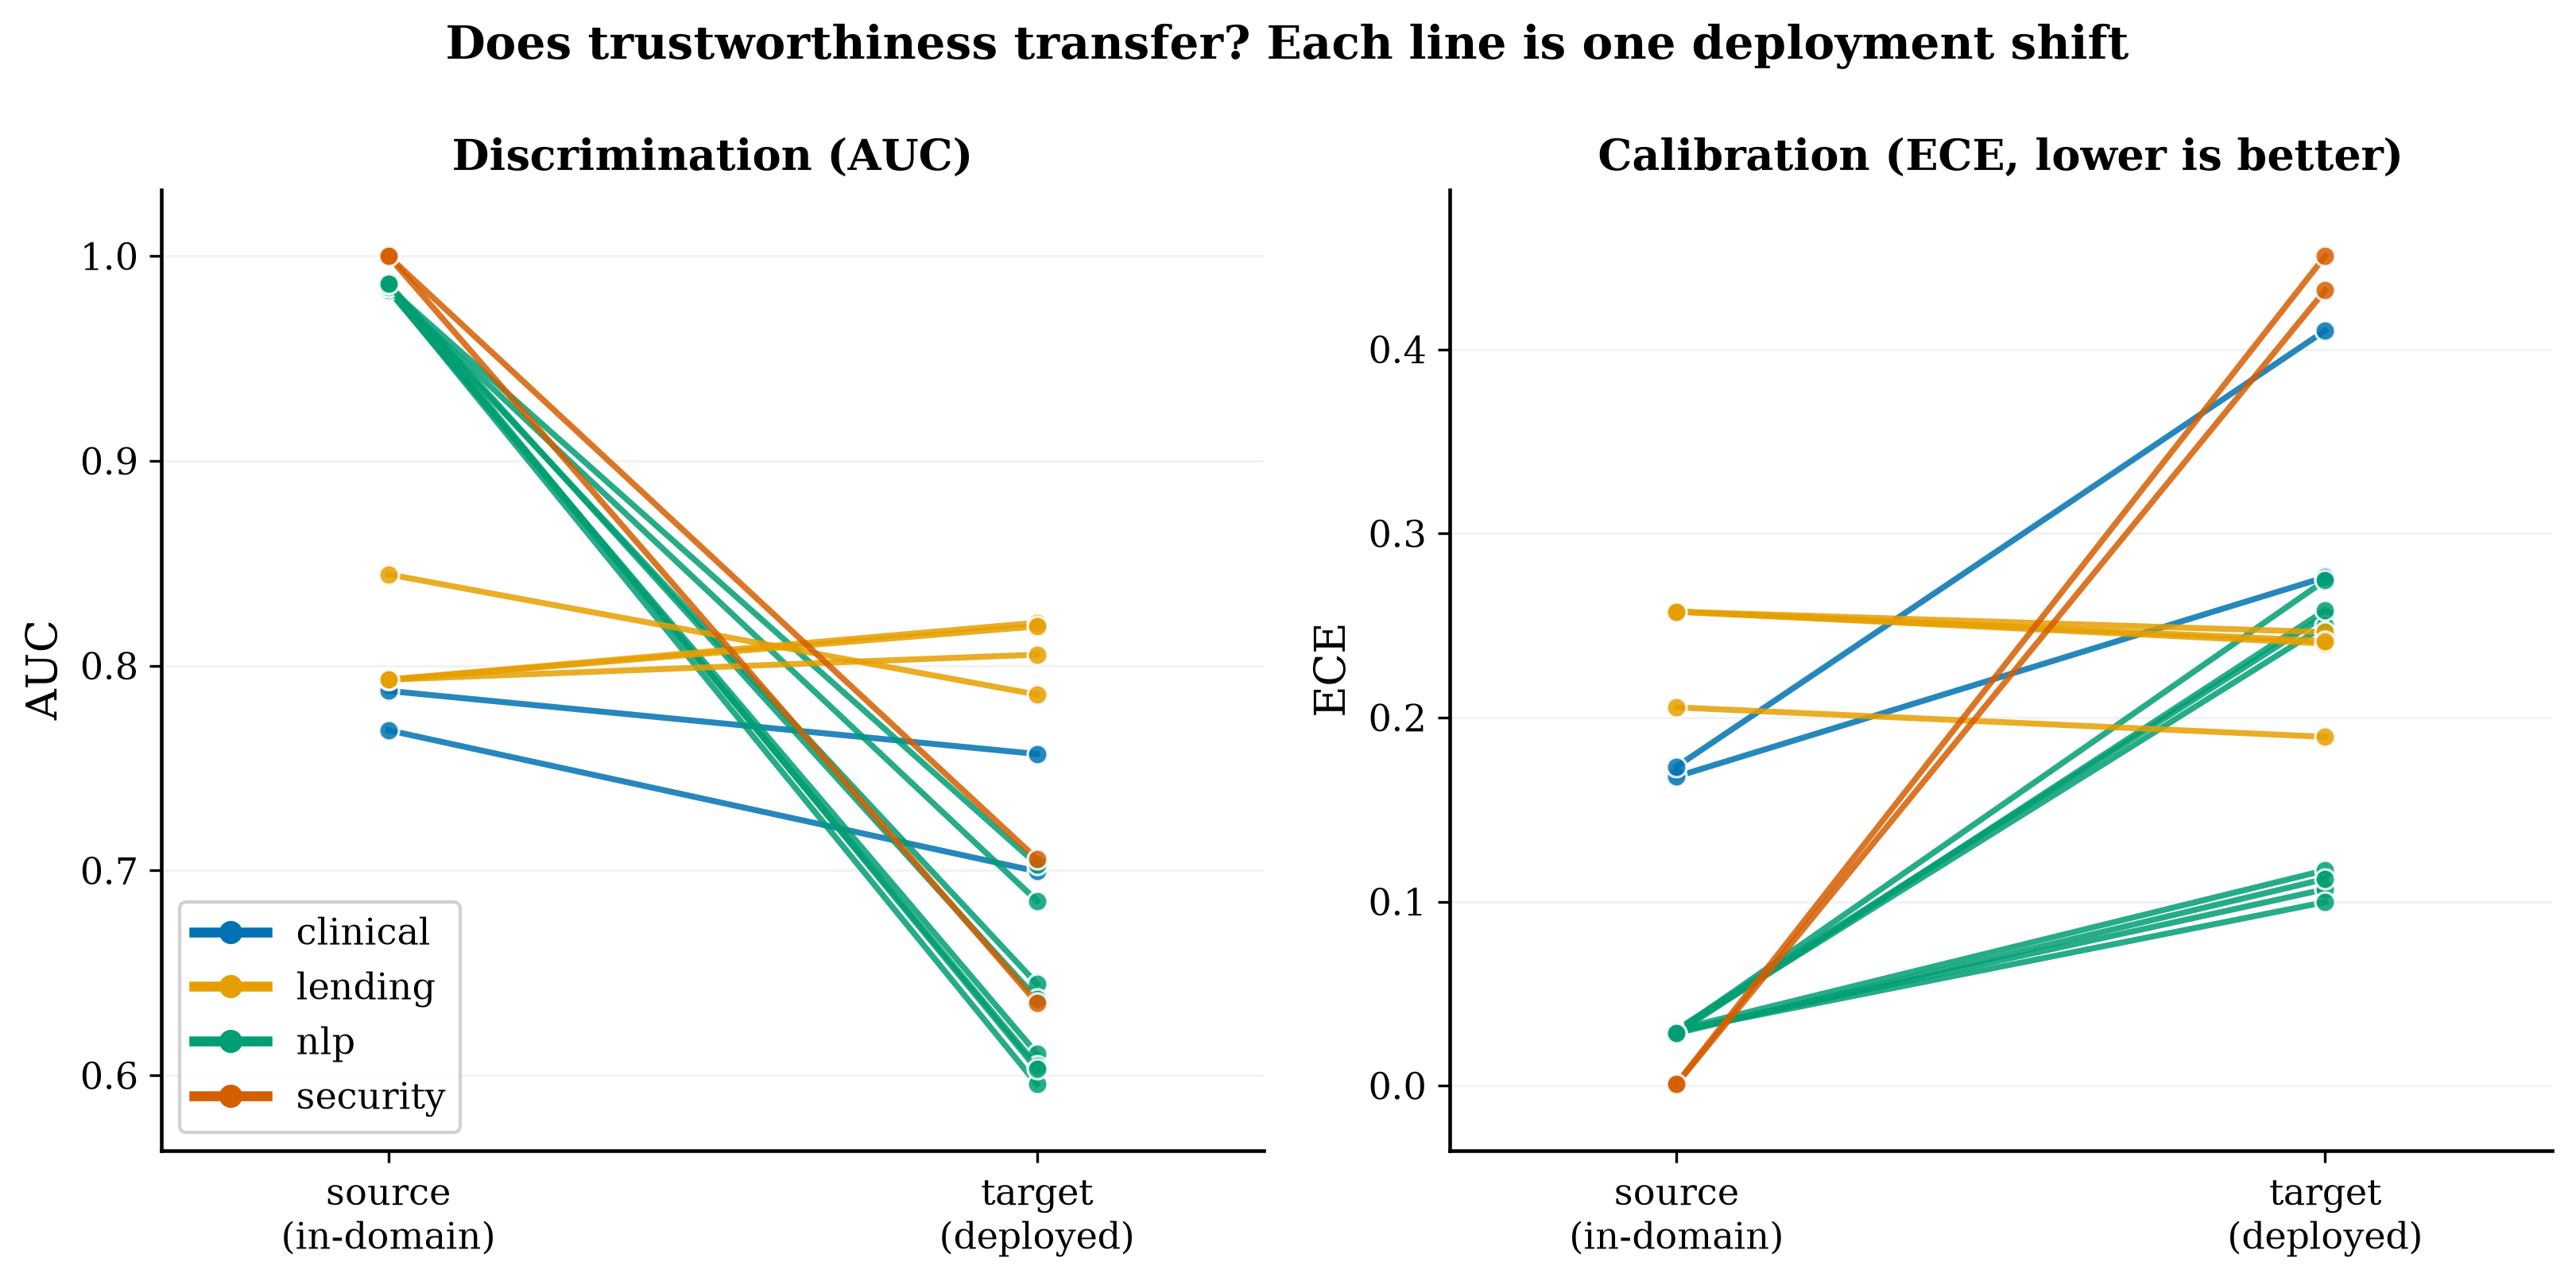
\includegraphics[width=\linewidth]{fig2_shift_bars.png}
\caption{Discrimination (left) and calibration (right) as each shift transfers: every line runs
from a shift-point's source (in-domain) value to its target (deployed) value, colored by domain.
Source values are high and uniform; target values fan out. Steep lines mark collapse (NLP, security
AUC), flat lines robustness (lending). The clinical lines are near-flat for AUC yet rise steeply for
ECE---calibration fails where discrimination does not.}
\label{fig:bars}
\end{figure}

\subsection{The failure is consistently predicted by the shift type (the taxonomy)}
\label{sec:res-fingerprint}

The four domains produce four distinct and interpretable failure fingerprints
(Table~\ref{tab:fingerprint}), and each fingerprint matches its mechanistic diagnosis.

\emph{Concept shift $\rightarrow$ everything fails.} The NLP shift diagnoses as concept shift:
the domain classifier separates platforms almost perfectly ($\text{AUC}_{\text{dc}} =
0.93$--$0.99$), yet importance-reweighting the source barely changes source AUC
($0.988\rightarrow 0.987$) while target AUC is $\approx 0.60$---covariate shift cannot explain the
drop. Discrimination collapses ($\Delta\text{AUC}$ $0.28$--$0.39$), calibration breaks (target ECE
up to $0.27$), and the subgroup gap widens ($\Delta G$ up to $+0.15$). All three axes fail together.

\emph{Novel-label shift $\rightarrow$ discrimination and calibration collapse on new classes.}
The intrusion detector achieves a perfect in-domain AUC of $1.00$ (a known separability property
of whole-flow DDoS features), then falls to $0.64$ externally, with ECE rising from $0.001$ to
$0.45$. The mechanism is label shift ($\Delta\pi = 0.34$): the deployment set contains attack
families absent from training. Per-family recall exposes it directly---families seen in training
are detected at $0.99$+, while novel families are nearly invisible (\texttt{hulk} $0.05$,
\texttt{slowhttp} $0.12$, \texttt{slowloris} $0.21$). A detector can be perfect in-domain and
blind to the attacks it will actually meet.

\emph{Covariate shift alone $\rightarrow$ no damage.} The lending temporal shift diagnoses as
covariate ($\text{AUC}_{\text{dc}}$ $0.69$--$0.80$) with no label or concept component, and nothing
fails: AUC \emph{improves} ($\Delta\text{AUC}$ $-0.012$ to $-0.028$), calibration is stable, and
the race gap shrinks. Geographic shift behaves the same (mild $\Delta\text{AUC}=+0.059$, gap
$-0.029$).

\emph{Mixed $\rightarrow$ silent calibration failure.} The clinical shift holds discrimination
($\Delta\text{AUC}=+0.031$) while calibration deteriorates sharply (ECE $0.168\rightarrow 0.276$
for the primary model; $0.41$ for the boosted baseline). The age subgroup gap does not widen; it
narrows ($\Delta G=-0.066$, 95\% CI $[-0.113,-0.016]$). A model whose AUC certifies it as
unchanged is producing risk estimates that are substantially miscalibrated.

\begin{table}[t]
\centering
\caption{\textbf{The failure fingerprint.} One row per domain (primary model). $\uparrow$/$\downarrow$
mark the direction and $\approx$ near-invariance. The trustworthiness axis that fails tracks the
diagnosis, across four dissimilar domains.}
\label{tab:fingerprint}
\small
\begin{tabular}{lccccc}
\toprule
Domain & Diagnosis & Discrimination & Calibration & Subgroup reliability \\
\midrule
NLP & concept & collapses ($\downarrow0.28$--$0.39$) & breaks & gap widens ($\uparrow$) \\
Security & novel-label & collapses ($1.00\!\rightarrow\!0.64$) & breaks ($\uparrow$ $450\times$) & novel-family blind \\
\rowcolor{hlrow} Clinical & mixed & \textbf{holds} ($\approx$) & \textbf{breaks silently} ($\uparrow$) & gap narrows ($\downarrow$) \\
Lending & covariate & holds/improves ($\approx$) & stable ($\approx$) & gap narrows ($\downarrow$) \\
\bottomrule
\end{tabular}
\end{table}

\begin{table}[t]
\centering
\caption{Master results, primary models. Source and target AUC/ECE, discrimination change, and
subgroup-gap change $\Delta G$ (positive = gap widens under shift). Numbers regenerate from
committed prediction files.}
\label{tab:master}
\scriptsize
\begin{tabular}{llcccccc}
\toprule
Domain & Target & AUC$_{\text{src}}$ & AUC$_{\text{tgt}}$ & $\Delta$AUC & ECE$_{\text{src}}$ & ECE$_{\text{tgt}}$ & $\Delta G$ \\
\midrule
\rowcolor{hlrow} Clinical & BRFSS & 0.788 & 0.757 & $+0.031$ & 0.168 & \textbf{0.276} & $-0.066$ \\
NLP & Reddit & 0.984 & 0.645 & $\mathbf{+0.339}$ & 0.030 & 0.117 & $+0.074$ \\
NLP & Twitter & 0.984 & 0.596 & $\mathbf{+0.388}$ & 0.030 & 0.255 & $+0.080$ \\
Lending & 2023 & 0.793 & 0.821 & $-0.028$ & 0.258 & 0.240 & $-0.031$ \\
Lending & held-out states & 0.845 & 0.786 & $+0.059$ & 0.206 & 0.190 & $-0.029$ \\
Security & CICIDS2017 & \textbf{1.000} & \textbf{0.635} & $\mathbf{+0.365}$ & 0.001 & \textbf{0.451} & --- \\
\bottomrule
\end{tabular}
\end{table}

\subsection{The regularity is categorical, not a magnitude law}\label{sec:meta}

Treating each (domain, model, target) as a shift-point ($n=16$), we asked whether the
subgroup-reliability change is predictable from cheaper quantities. \emph{Because the observations
cluster strongly by domain (effectively four clusters), we interpret every regression in this
section as an exploratory cross-domain summary, not a fitted predictor.} With that caveat stated
first: across shift-points, gap change is associated with calibration change (slope $0.42$, 95\% CI
$[0.17,0.60]$, $R^2=0.41$) and with aggregate accuracy loss (slope $0.34$, CI $[0.27,0.44]$,
$R^2=0.82$). The tempting third association---subgroup loss with covariate-shift magnitude---has a
high cross-domain fit (slope $0.54$, $R^2=0.77$) but is a statistical trap, which we report against
ourselves.

\begin{tcolorbox}[colback=gray!6,colframe=gray!50,title=\textbf{Unexpected finding: shift
magnitude is not deployment damage}]
The cross-domain regression of subgroup-gap change on covariate-shift magnitude
($\text{AUC}_{\text{dc}}$) has slope $+0.54$ with $R^2=0.77$---a fit that, taken at face value,
would license ``measure the shift; the bigger it is, the more subgroup reliability you lose.''
That reading is wrong. Within the lending domain, where covariate-shift magnitude rises from
$0.69$ to $0.80$ across deployment years, the same slope is \emph{negative} ($-0.10$): more
measured shift, less damage. The positive cross-domain slope is a two-cluster (Simpson) artifact
separating high-shift text from moderate-shift tabular data---an aggregate line drawn through two
groups that individually tell the opposite story. Lending exhibits larger measured covariate shift
than many settings described as ``severe,'' while remaining fully robust on every axis. This
mattered to our own analysis: an earlier version of this work reported the $0.54$ slope as a
finding before the within-domain check exposed it, and we retain it here precisely because the
mistake is instructive. \textbf{Shift magnitude and deployment risk are not interchangeable}; the
\emph{categorical} diagnosis (Figure~\ref{fig:taxonomy}), recoverable from cheap probes, is what
tracks failure.
\end{tcolorbox}

We therefore report the cross-domain regressions (Figure~\ref{fig:scatter}) as exploratory
synthesis over four domain-clusters, not as a fitted predictor, and rest the contribution on the
categorical taxonomy.

\begin{figure}[t]
\centering
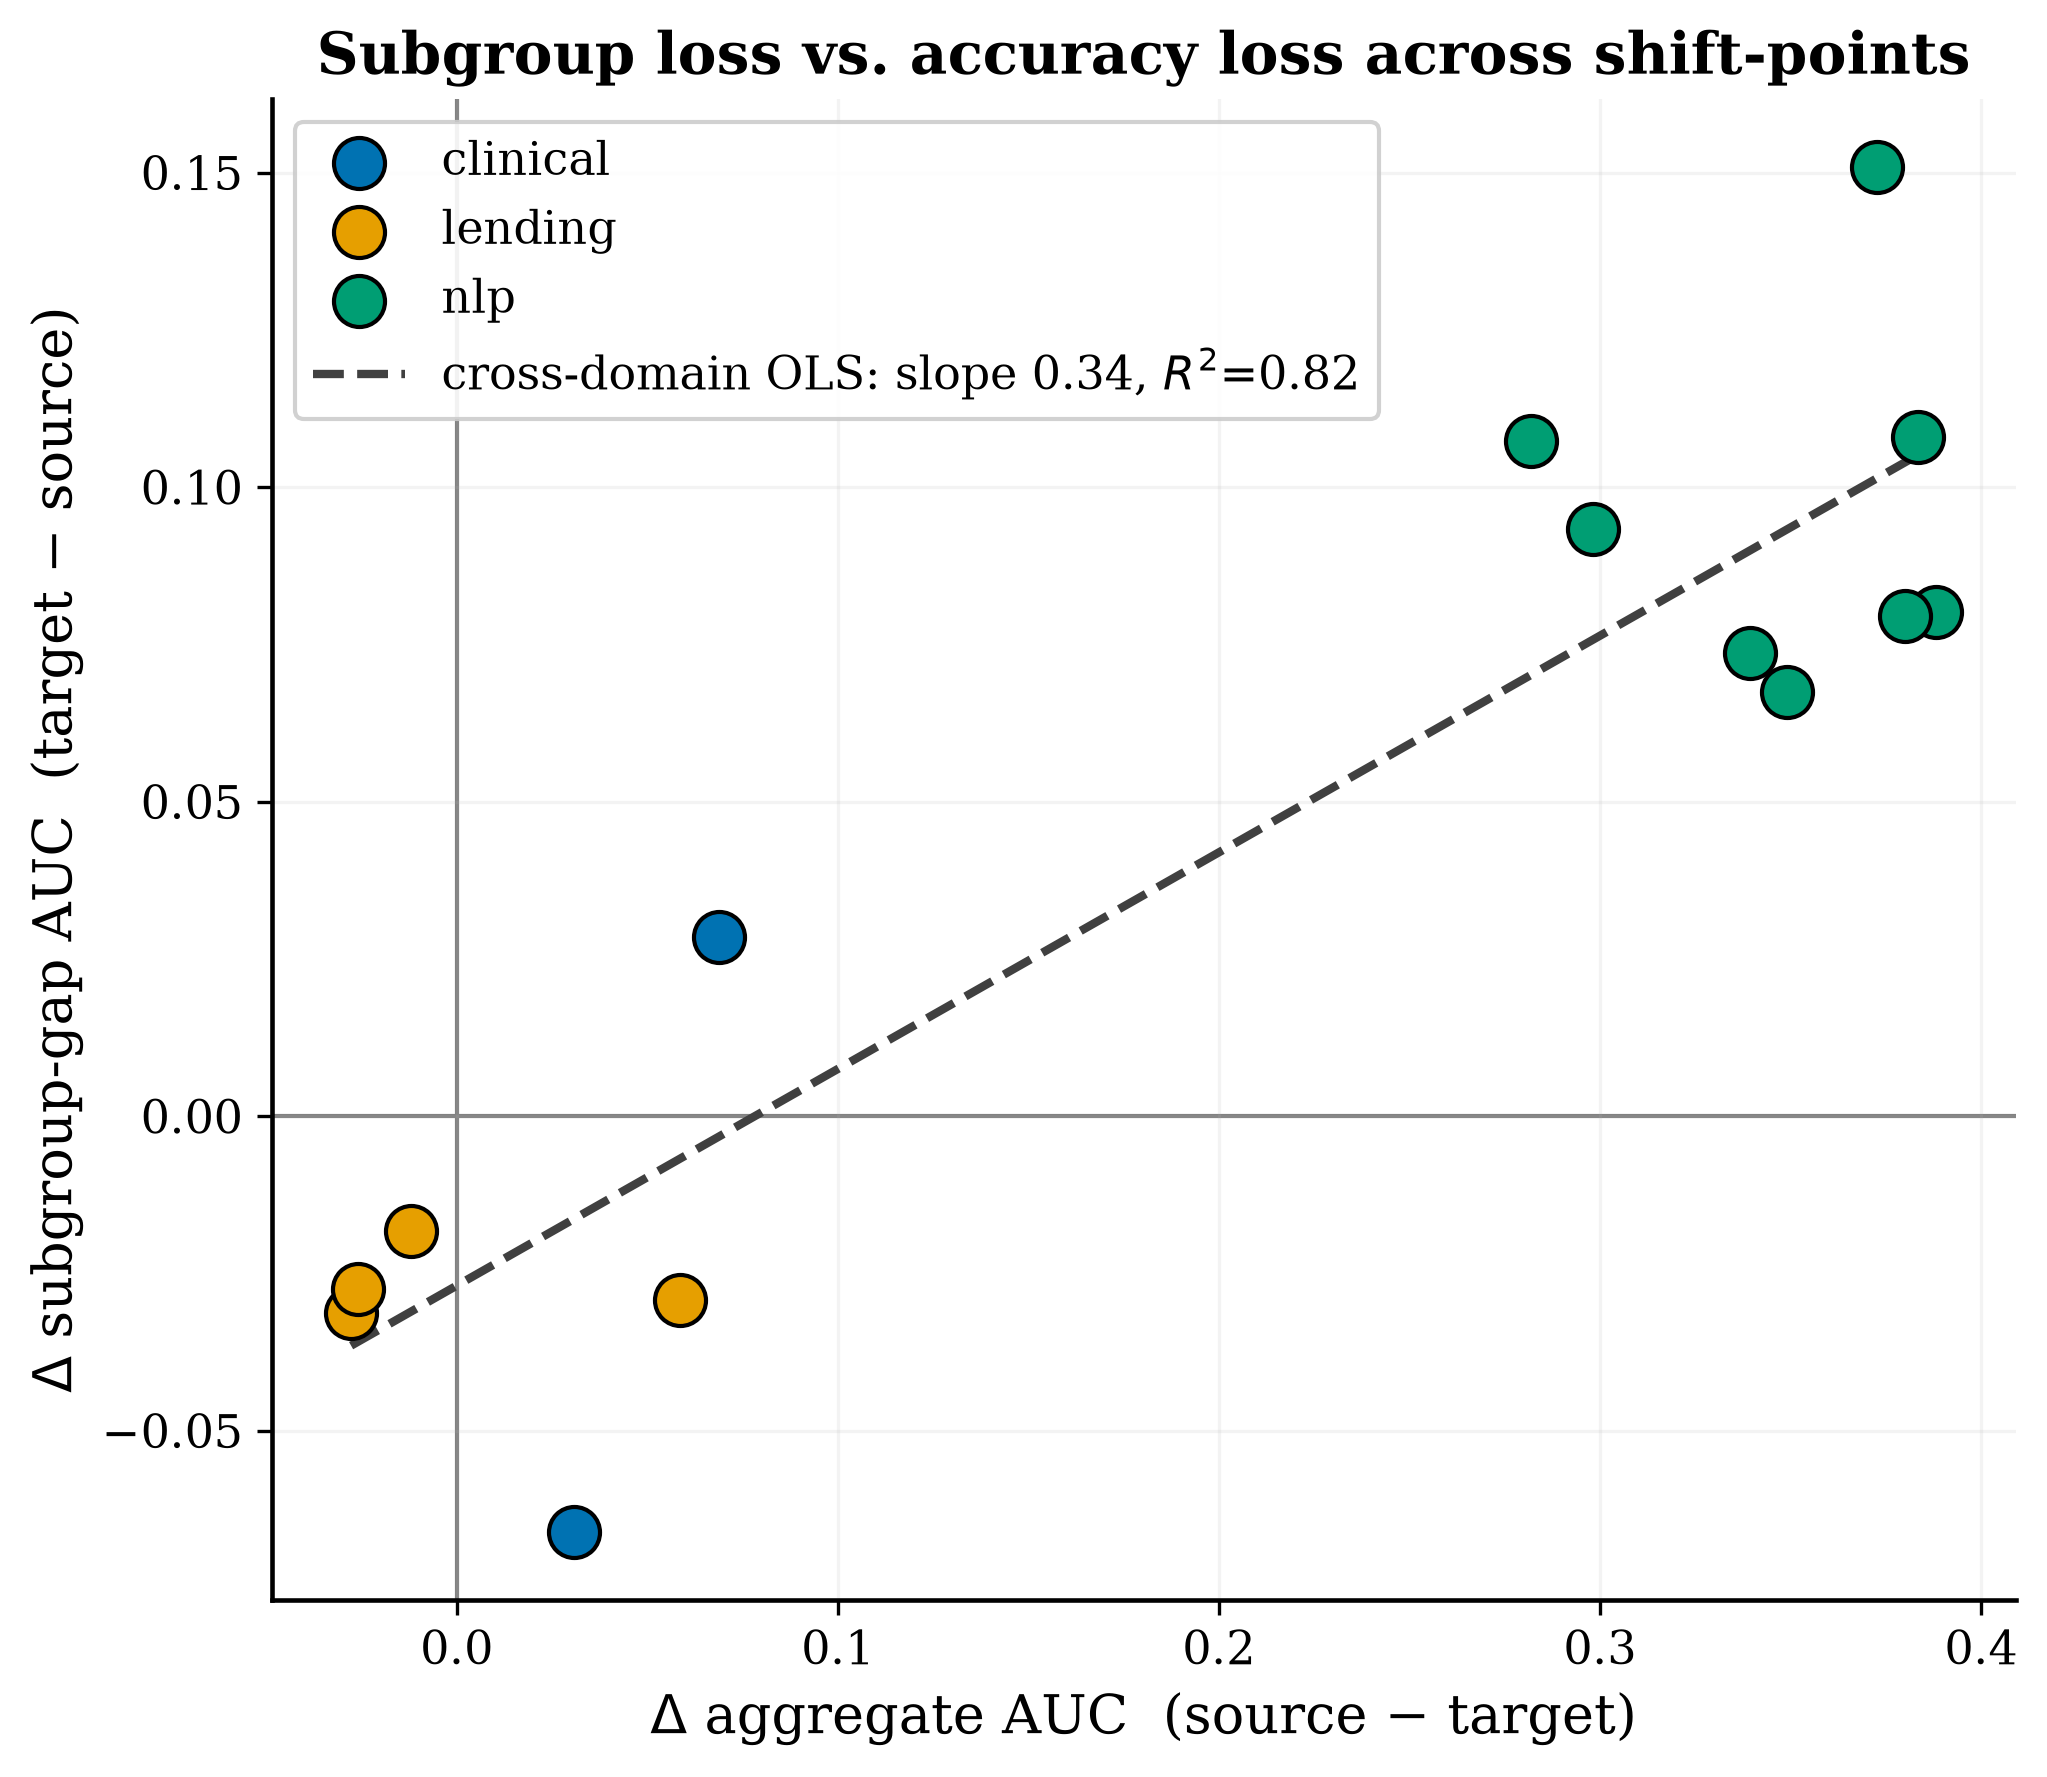
\includegraphics[width=0.7\linewidth]{fig3_headline_scatter.png}
\caption{Subgroup-gap change vs.\ aggregate accuracy loss across shift-points, colored by domain.
The cross-domain trend is real but domain-clustered; within-domain slopes differ (see box).
Security is absent because its operational subgroups are all-positive, so a gap is undefined.}
\label{fig:scatter}
\end{figure}

\subsection{Recalibration repairs calibration only}\label{sec:res-remediation}

Isotonic recalibration on a 10\% labeled target split reduced ECE by one to two orders of
magnitude in every domain: clinical $0.276\rightarrow 0.002$, lending $0.246\rightarrow 0.006$,
security $0.450\rightarrow 0.013$, NLP $0.115/0.254\rightarrow 0.016/0.055$
(Table~\ref{tab:remediation}). In the three continuous-score domains, AUC and the subgroup gap
moved by less than $0.012$---calibration is cheaply repairable, discrimination and reliability are
not. (For security the isotonic map perturbs AUC by $+0.07$; because the in-domain-perfect
detector emits near-degenerate probabilities, isotonic collapses them into $28$ tied levels, and
AUC with heavy ties is not transform-invariant. This is a tie artifact, not restored
discrimination: $+0.07$ does not recover the $0.37$ collapse.) Restoring discrimination requires
target supervision---e.g., in the NLP domain, target fine-tuning recovers far more than any
post-hoc fix~\citep{pall2026cpfe}.

\begin{table}[t]
\centering
\caption{Remediation ladder (isotonic recalibration on 10\% target labels). ECE falls sharply;
AUC is essentially unchanged in continuous-score domains.}
\label{tab:remediation}
\small
\begin{tabular}{llcccc}
\toprule
Domain & Target & ECE (no fix) & ECE (isotonic) & AUC (no fix) & AUC (isotonic) \\
\midrule
Clinical & BRFSS & 0.276 & 0.002 & 0.757 & 0.757 \\
Lending & 2023 & 0.240 & 0.002 & 0.821 & 0.821 \\
NLP & Twitter & 0.254 & 0.055 & 0.592 & 0.589 \\
Security & CICIDS2017 & 0.450 & 0.013 & 0.634 & 0.708$^{\dagger}$ \\
\bottomrule
\end{tabular}
\captionsetup{font=footnotesize}
\caption*{$^{\dagger}$ tie artifact from near-degenerate scores; not restored discrimination.}
\end{table}

\section{Discussion}\label{sec:discussion}

\paragraph{What failed, and why.} The four domains failed in four ways, and each way matched its
shift mechanism. Concept shift (NLP) broke every axis because the input--label relationship itself
changed. Novel-label shift (security) broke discrimination and calibration precisely on classes
absent from training, leaving trained classes untouched. Covariate shift alone (lending) broke
nothing, even at large magnitude. Mixed shift (clinical) broke calibration while sparing
discrimination. The common thread is mechanistic: the axis that fails is the axis the shift
mechanism attacks.

\paragraph{The most practically important observation.} Maintaining high discrimination after
deployment did not imply trustworthy behaviour. The clinical model retained its AUC while its
probability estimates became substantially miscalibrated, and the lending model stayed robust
despite measurable covariate shift. These contrasting outcomes argue that deployment decisions
should not rest on aggregate discrimination alone, but should incorporate diagnostics tailored to
the underlying shift mechanism---which are cheap and, for covariate and label probes, require no
target labels.

\paragraph{What practitioners should do differently.} The results support a concrete
pre-deployment routine: (1) probe label prevalence; (2) fit a source-vs-target domain classifier;
(3) run the reweighting probe. The resulting diagnosis indicates which dashboard will mislead---a
covariate-only diagnosis is reassuring, a concept or novel-label diagnosis is a warning that
discrimination and subgroup reliability, not just calibration, are at risk---and a small labeled
target sample should be budgeted for recalibration, which was cheap and universally effective.
Monitoring aggregate AUC alone, the most common practice, was the least informative signal in all
four domains.

\paragraph{Outlook.} If this pattern continues to hold across additional domains, deployment
evaluation may need to shift its emphasis from measuring \emph{how large} a distribution shift is
toward identifying \emph{what type} of shift has occurred before deployment. We do not claim a
universal law from four domains; we claim a reproducible regularity, a mechanism that explains it,
and a cheap protocol for testing whether it holds in a new setting. Establishing its boundaries---the
domains, shift types, and model classes where the taxonomy breaks down---is the natural next step,
and the benchmark is built to accept new domains.

\section{Related Work}\label{sec:related}

\paragraph{Shift benchmarks} such as WILDS~\citep{koh2021wilds} and
TableShift~\citep{gardner2023tableshift} quantify how much accuracy drops under shift, within a
modality. TrustShift differs in measuring calibration and subgroup reliability alongside
discrimination, in assigning a mechanistic diagnosis, and in spanning modalities so cross-domain
regularities are visible.

\paragraph{Fairness under shift} has been examined mostly in single domains; \citet{schrouff2022diagnosing}
show fairness properties fail to transfer in medical settings and that clinically plausible shifts
violate the assumptions of single-mechanism mitigations. We corroborate the multi-mechanism point
across four domains and connect the mechanism to which axis fails. A recent
survey~\citep{lin2024fairnessshiftsurvey} catalogues methods; we contribute an empirical taxonomy.

\paragraph{Shift diagnosis and calibration.} Our probes build on black-box shift
detection~\citep{rabanser2019failing}, label-shift estimation~\citep{lipton2018label}, and
post-hoc calibration~\citep{guo2017calibration,zadrozny2002isotonic}. Our contribution is not a new
estimator but the finding that these cheap diagnostics, applied jointly, predict \emph{which}
trustworthiness axis a deployment will break.

\section{Limitations}\label{sec:limitations}

Four domains and sixteen shift-points are evidence, not proof; the cross-domain regressions are
exploratory synthesis over effectively four clusters, and we do not present them as a fitted
predictor. Subgroup semantics differ across domains by necessity---demographic for clinical and
lending, platform-derived proxy classes for text, and \emph{operational} attack families for
security---and we never interpret security's subgroup reliability as demographic fairness.
Clinical target-side subgroup analysis is limited to age: the released prediction arrays were
generated from a previously harmonized BRFSS dataset whose preprocessing pipeline is no longer
recoverable, so sex, race, and BMI analyses are not reproducible on the target side; age-based
analyses remain fully reproducible and constitute the primary clinical subgroup evaluation. The
clinical and lending subgroup gaps \emph{narrow} under shift, which we attribute tentatively to
changes in subgroup composition rather than to genuine fairness improvement, and flag as a
hypothesis. The security detector's near-perfect in-domain AUC is a known separability property of
whole-flow features, which we treat as the in-domain ceiling rather than a result. This study
examines four deployment settings rather than an exhaustive sample of machine-learning domains;
important modalities---especially vision foundation models and large language models, whose shift
behaviour may differ---remain to be tested, and the benchmark is designed to accept them.
Finally, all experiments run on a single workstation, bounding model scale.

\section{Conclusion}\label{sec:conclusion}

Deployment shift does not degrade machine-learning trustworthiness uniformly. Which axis
fails---discrimination, calibration, or subgroup reliability---is set by the type of shift, and the
type is recoverable before deployment with cheap, largely label-free diagnostics; the magnitude of
shift is not, on its own, a measure of risk. In-domain metrics predicted none of this. We make the
TrustShift protocol and benchmark available upon publication so that new domains can be placed on
the same axes, and offer the resulting taxonomy as a practical guide to what a deployment audit
should check.

\section*{Data and Code Availability}
The TrustShift protocol, the four domain adapters, the audit engine, and every results file that
backs a number in this paper---together with a single script that regenerates all tables and
figures from the committed prediction files---will be made publicly available upon publication as an
open-source repository and an accompanying benchmark of harmonized predictions, with a versioned,
DOI-citable archive; anonymized access can be provided to reviewers on request. All source datasets
are public (NHANES, BRFSS, HMDA, GoEmotions, CIC-DDoS2019, CICIDS2017); consistent with their
licenses we redistribute standardized model predictions and metadata, not raw third-party records.
Seeds, estimator settings, and metric definitions are fixed in the accompanying configuration.

\bibliography{references}

\end{document}
